\documentclass[journal,12pt,twocolumn]{IEEEtran}
\usepackage{cite}
\usepackage{amsmath,amssymb,amsfonts,amsthm}
\usepackage{algorithmic}
\usepackage{graphicx}
\usepackage{textcomp}
\usepackage{xcolor}
\usepackage{txfonts}
\usepackage{listings}
\usepackage{enumitem}
\usepackage{mathtools}
\usepackage{float}
\usepackage{gensymb}
\usepackage{comment}
\usepackage[breaklinks=true]{hyperref}
\usepackage{tkz-euclide} 
\usepackage{listings}
\usepackage{gvv}                                        
\def\inputGnumericTable{}                                 
\usepackage[latin1]{inputenc}                                
\usepackage{color}                                            
\usepackage{array}                                            
\usepackage{longtable}                                       
\usepackage{calc}                                             
\usepackage{multirow}                                         
\usepackage{hhline}                                           
\usepackage{ifthen}                                           
\usepackage{lscape}
\usepackage{amsmath}
\usepackage{subcaption}
\newtheorem{theorem}{Theorem}[section]
\newtheorem{problem}{Problem}
\newtheorem{proposition}{Proposition}[section]
\newtheorem{lemma}{Lemma}[section]
\newtheorem{corollary}[theorem]{Corollary}
\newtheorem{example}{Example}[section]
\newtheorem{definition}[problem]{Definition}
\newcommand{\BEQA}{\begin{eqnarray}}
\newcommand{\EEQA}{\end{eqnarray}}
\newcommand{\define}{\stackrel{\triangle}{=}}
\theoremstyle{remark}
\newtheorem{rem}{Remark}
\usepackage{tikz}
\usepackage{circuitikz} 

\begin{document}

\bibliographystyle{IEEEtran}
\vspace{3cm}

\title{NCERT Analog- 12.7.7}
\author{EE23BTECH11045 - Palavelli Srija$^{*}$}

\maketitle

\bigskip

\renewcommand{\thefigure}{\theenumi}
\renewcommand{\thetable}{\theenumi}

\vspace{3cm}
\textbf{Question 12.7.7:} 
Let $x(t) = 10 \cos(10.5 \omega t)$ be passed through an LTI system with impulse response $h(t) = \pi\left(\frac{\sin(\omega t)}{\pi t}\right)^2 \cos(10 \omega t)$ . The output of the system is:\\ \hfill(GATE EC 2023)\\
\textbf{Solution}\\
Given \(h(t)\) is Real and Even. When a sinusoidal input is applied to an LTI system with an even impulse response, the output will also be sinusoidal.
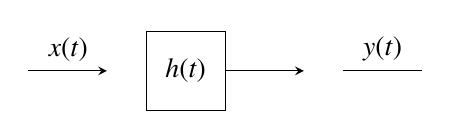
\begin{tikzpicture}[>=stealth]
	\centering
    % x(t) outside rectangle
    \draw[->] (0,0) -- node[above] {$x(t)$} (1,0);
    
    % h(t) inside rectangle
    \draw (1.5,-0.5) rectangle node {$h(t)$} (2.5,0.5);
    \draw[->] (2.5,0) -- (3.5,0);
    
    % y(t) without the line under it
    \draw (4,0) -- node[above] {$y(t)$} (5,0);
\end{tikzpicture}
\begin{align}
y(t) &= H(\omega)\bigg|_{\omega=10.5\omega} \cdot 10 \cos(10.5 \omega t) \\
h(t) &= f(t) \cos(10 \omega t) \\
f(t) &= \pi\left(\frac{\sin(\omega t)}{\pi t}\right)^2 \\
\end{align}

The Fourier transform of \(f(t)\):
\begin{align} 
f(t) \xleftrightarrow{\mathcal{F}} F(\omega)\\
 F(\omega)&= \pi\int_{-\infty}^{\infty}\left(\frac{\sin(\omega t)}{\pi t}\right)^2e^{-j\omega t}\,dt 
\end{align}
\begin{figure}[h!]
    \centering
    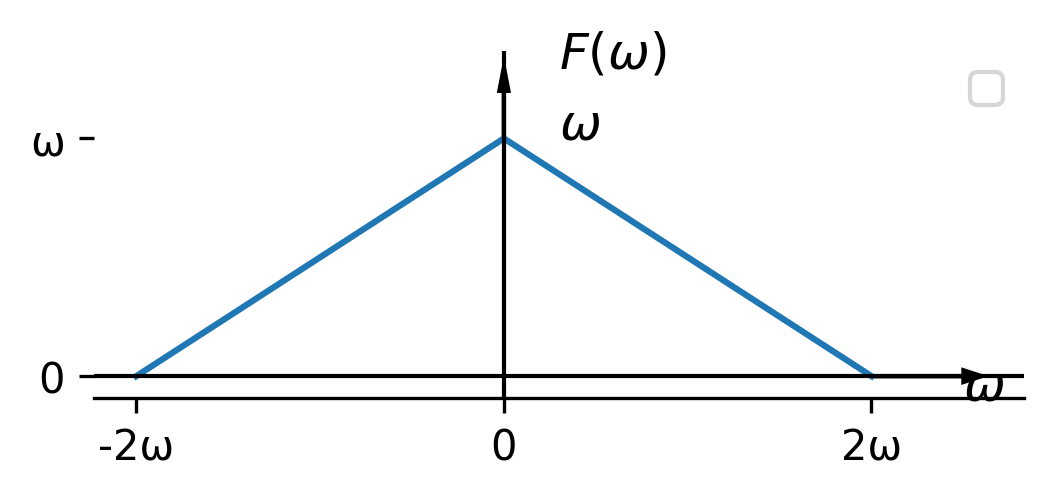
\includegraphics[width=\columnwidth]{figs/plot2.png}
    \caption{}
    \label{fig:sr2}
\end{figure}

\begin{enumerate}
The frequency response \(H(\omega)\):
\end{enumerate}
\begin{align}
H(\omega) &= \frac{1}{2} \left[F(\omega + 10\omega) + F(\omega - 10\omega)\right] 
\end{align}
\begin{figure}[h!]
    \centering
    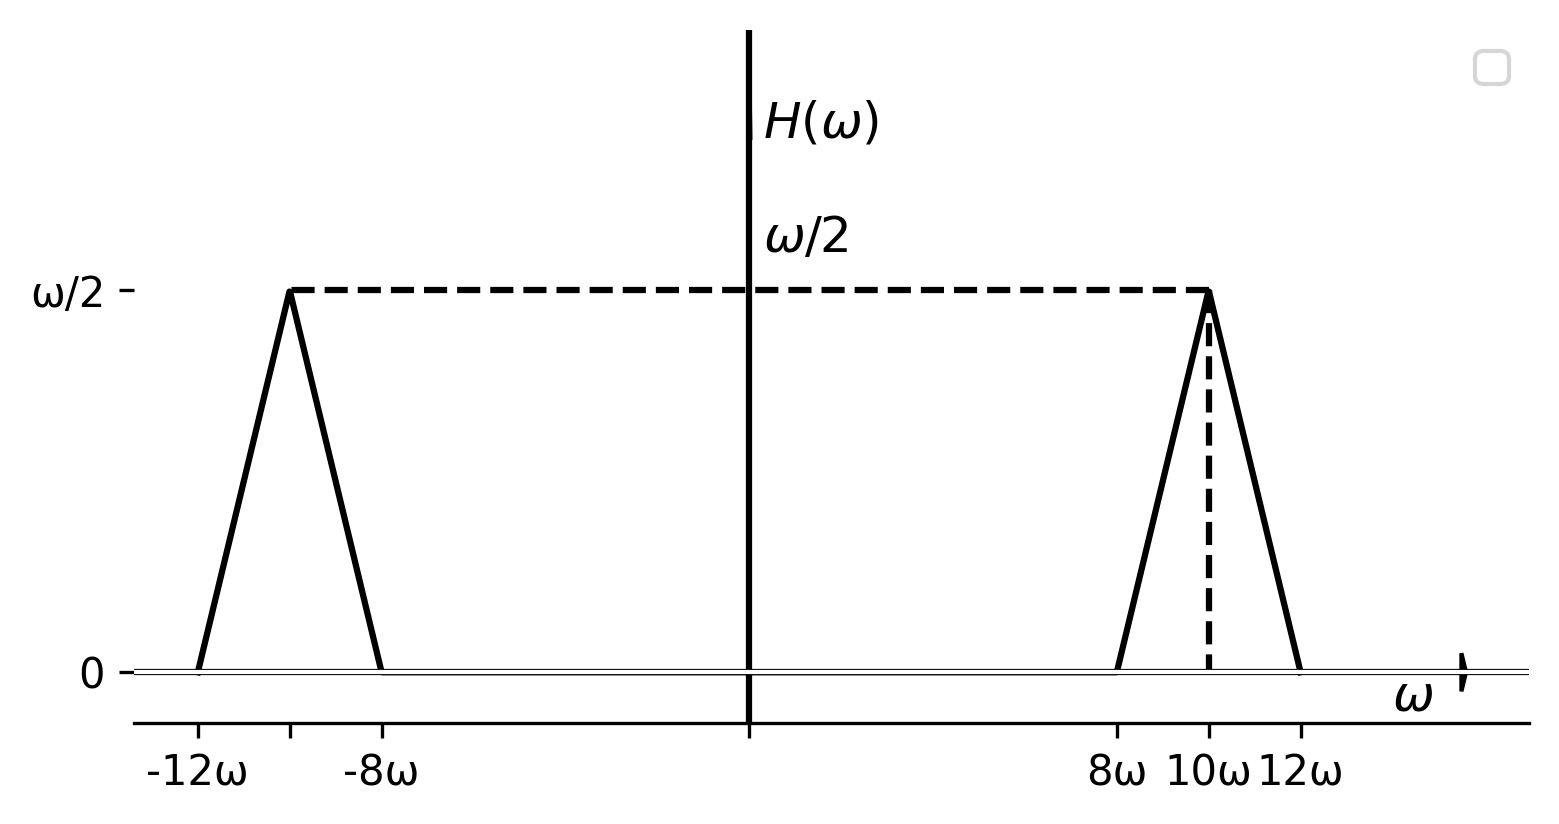
\includegraphics[width=\columnwidth]{figs/plot3.png}
    \caption{}
    \label{fig:sr3}
\end{figure}
\begin{align}
H(\omega)\bigg|_{\omega=10.5\omega} = \frac{3}{8}\omega
\end{align}
The output \(y(t)\):
\begin{align}
y(t) &= \frac{3}{8}\omega \cdot 10 \cos(10.5 \omega t) \\
&= \frac{15}{4}\omega \cos(10.5 \omega t)
\end{align}

\end{document}


